We use the fixed-effects regression model to estimate the effect size of these characteristics on the total duration of the case. A fixed-effects regression model is an estimation technique that allows one to control for time-invariant unobserved variables that can be correlated with the observed characteristics, thus allowing us to estimate the effect size of identified (observed) characteristics on the total duration of cases. Notably, we only rely on disposed cases since pending cases in our data often do not have interim orders. By definition, they also do not have a final order. Thus, including such cases in the estimation can lead to higher uncertainty. For the empirical analysis, we only used the 37,498 disposed cases. 

While hazard models, on the lines of \textcite{datta2017_itatDelays}, would be an ideal choice to use in such an analysis, we chose the fixed-effects model due to the peculiarities of our data. Case-characteristics for pending cases cannot be reliably detected because orders for those cases are not available in most instances. Further, given that most cases in our data-set are disposed, we did not expect significantly different results from using a fixed-effects model. Finally, a fixed-effects model gives coefficients that can be easily interpreted, whereas hazard models yield probabilities for a case to conclude after a given duration. The coefficient from the fixed-effects model is therefore easier to for policy reform than the results of a hazard model.

Table \ref{tab:disposal_regression} shows the results of the fixed effects regression to predict the effects on total case duration (in days). The State in which the case is filed has a large and statistically significant effect on the case duration. Controlling for the State-level effects, all but one of the selected case characteristics significantly increase the case duration.

\begin{table}
\centering
 \caption{Effect of case characteristics on days required to dispose a case}\label{tab:disposal_regression}
 \footnotesize \scalebox{0.97}{ \hspace*{-0.6cm}
 \begin{tabular}{lccccccc}
 \\[-1.8ex]
 \hline \\[-1.8ex] 
 & \multicolumn{7}{c}{\textit{Dependent variable: Disposal Days}} \\ 
 \cline{2-8} 
 \\[-1.8ex] & (1) & (2) & (3) & (4) & (5) & (6) & (7)\\ 
 \hline \\[-1.8ex] 
 D(non-Appearance) & 265.271$^{***}$ & & & & & & 200.695$^{***}$ \\ 
 & (5.184) & & & & & & (4.979) \\ 
 & & & & & & & \\ 
 D(Summons) & & 178.660$^{***}$ & & & & & 112.250$^{***}$ \\ 
 & & (5.322) & & & & & (5.214) \\ 
 & & & & & & & \\ 
 D(Mediation) & & & 161.640$^{***}$ & & & & 100.383$^{***}$ \\ 
 & & & (5.338) & & & & (4.971) \\ 
 & & & & & & & \\ 
 D(Jurisdiction) & & & & 309.402$^{***}$ & & & 271.877$^{***}$ \\ 
 & & & & (5.138) & & & (4.921) \\ 
 & & & & & & & \\ 
 D(Multiplicity) & & & & & 271.545$^{***}$ & & 168.070$^{***}$ \\ 
 & & & & & (10.117) & & (9.938) \\ 
 & & & & & & & \\ 
 D(Contested) & & & & & & 0.200 & $-$53.246$^{***}$ \\ 
 & & & & & & (5.614) & (5.351) \\
 \hline \\[-1.8ex] 
 State FE & Y & Y & Y & Y & Y & Y & Y \\ 
 Year FE & Y & Y & Y & Y & Y & Y & Y \\
 \hline \\[-1.8ex] 
 Observations & 35,427 & 35,427 & 35,427 & 35,427 & 35,427 & 35,427 & 35,427 \\ 
 R$^{2}$ & 0.137 & 0.102 & 0.097 & 0.159 & 0.092 & 0.073 & 0.241 \\ 
 Adjusted R$^{2}$ & 0.137 & 0.101 & 0.096 & 0.159 & 0.091 & 0.073 & 0.241 \\
 \hline \\[-1.8ex] 
 \textit{Note:} & \multicolumn{7}{r}{$^{*}$p$<$0.1; $^{**}$p$<$0.05; $^{***}$p$<$0.01} \\ 
 \end{tabular}}
\end{table}

As with the total duration to dispose the cases, the State in which the case is filed has a large and statistically significant effect on the number of hearings. 


Table \ref{tab:hearings_regression} shows the results of the fixed-effects regression to estimate the effect of case characteristics on the number of hearings required to dispose the case. Controlling for the State-level effects, all of the selected case characteristics significantly increase the number of hearings required to dispose the case.

{\footnotesize
 \begin{longtable}{lccccccc}
 \caption{Effect of case characteristics on hearings required to dispose a case}\label{tab:hearings_regression}\\
 \\[-1.8ex]
 \hline \\[-1.8ex] 
 & \multicolumn{7}{c}{\textit{Dependent variable: Number of hearing (for disposed cases only)}} \\ 
 \cline{2-8} 
 \\[-1.8ex] & (1) & (2) & (3) & (4) & (5) & (6) & (7)\\ 
 \hline \\[-1.8ex]
 D(non-Appearance) & 9.641$^{***}$ & & & & & & 7.049$^{***}$ \\ 
 & (0.146) & & & & & & (0.131) \\ 
 & & & & & & & \\ 
 D(Summons) & & 11.031$^{***}$ & & & & & 7.368$^{***}$ \\ 
 & & (0.145) & & & & & (0.138) \\ 
 & & & & & & & \\ 
 D(Mediation) & & & 5.605$^{***}$ & & & & 3.200$^{***}$ \\ 
 & & & (0.153) & & & & (0.131) \\ 
 & & & & & & & \\ 
 D(Jurisdiction) & & & & 6.985$^{***}$ & & & 5.471$^{***}$ \\ 
 & & & & (0.151) & & & (0.130) \\ 
 & & & & & & & \\ 
 D(Multiplicity) & & & & & 17.460$^{***}$ & & 9.926$^{***}$ \\ 
 & & & & & (0.280) & & (0.262) \\ 
 & & & & & & & \\ 
 D(Contested) & & & & & & 6.218$^{***}$ & 2.889$^{***}$ \\ 
 & & & & & & (0.159) & (0.141) \\ 
 \hline \\[-1.8ex]
 State FE & Y & Y & Y & Y & Y & Y & Y \\ 
 Year FE & Y & Y & Y & Y & Y & Y & Y \\ 
 \hline \\[-1.8ex] 
 Observations & 35,427 & 35,427 & 35,427 & 35,427 & 35,427 & 35,427 & 35,427 \\ 
 R$^{2}$ & 0.178 & 0.207 & 0.110 & 0.129 & 0.168 & 0.115 & 0.368 \\ 
 Adjusted R$^{2}$ & 0.177 & 0.207 & 0.110 & 0.129 & 0.168 & 0.115 & 0.367 \\ 
 \hline \\[-1.8ex] 
 \textit{Note:} & \multicolumn{7}{r}{$^{*}$p$<$0.1; $^{**}$p$<$0.05; $^{***}$p$<$0.01} \\ 
\end{longtable}}

The results for each of the case characteristics are discussed in detail in the following sub-sections.

\subsection{Non-appearance of accused}
\label{sec:non-appe-accus-1}

The results, shown in Table \ref{tab:summary_results}, indicate that non-appearance of the accused typically adds 213 days to the total case duration. Further, non-appearance of the accused typically adds 7 hearings to the total hearings required to dispose a case. Both these findings are in line with what we expected.

Therefore, any interventions by courts to ensure the accused's presence will help reduce the case durations and the number of hearings to dispose. The suggested interventions include serving notice of summons through digital media, such as instant messaging, email, and the Supreme Court's automated notice-service software.

Ordinarily, if the accused fails to appear before the court repeatedly, the court issues a bailable warrant to produce them in court. If the accused still fails to appear, the court issues a non-bailable warrant under \S~70 of the Code of Criminal Procedure (CrPC). This gives the police the power to arrest the accused anytime and anywhere. The police are also given the authority to forcibly open or break down the doors and walls of the home or the hiding place of the accused. If the accused still fails to appear in court even after the arrest warrants have been issued without bail, the judge can declare the accused to be a ``criminal accused'' under \S\S~82 and 83 of the CrPC. It can then authorise the attachment and sale of the accused's property to recover the disputed amount. One way of reducing delays caused due to the non-appearance may to reduce the time taken to conduct such processes, compelling the accused's presence.

\subsection{Jurisdictional issues}
\label{sec:jurisd-issu}

The results, shown in Table \ref{tab:summary_results}, indicate that jurisdictional issues typically add 287 days to the total case duration. Further, jurisdictional issues typically add 5.7 hearings to the total hearings required to dispose a case. Both these findings are in line with what we expected.

\subsection{Conversion to summons trial}
\label{sec:conv -summ-trial-1}

The results, shown in Table \ref{tab:summary_results}, indicate that conversion to a summons trial typically adds 111 days to the total case duration. Further, conversion to a summons trial typically adds 7.2 hearings to the total hearings required to dispose a case. Both these findings are in line with what we expected.

The Supreme Court and the Amici Curiae recommend that most cases be tried summarily. If courts implement this, they can significantly reduce the duration of cheque dishonour cases. The mechanism that the Supreme Court proposes is for courts to not convert cases to summons trials unless the accused presents a plausible defence. Further, the court has to record, in writing, its reasons for conducting the case as a summons trial. This recommendation, by itself, may be of limited use, unless an audit mechanism is put in place to assess how often and for what reason cases are converted to summons trials, and whether it was necessary to do so. This will also necessitate institutionalising a mechanism for regular judicial impact assessments.

\subsection{Cases referred to mediation}
\label{sec:mediation}

The results, shown in Table \ref{tab:summary_results}, indicate that a case being referred to mediation typically adds 108 days to the total time required to dispose it. Further, the case being referred to mediation typically adds 3.3 hearings to the number of hearings required to dispose the case. These findings run counter to our hypotheses that cases referred to mediation take less time and fewer hearings to dispose. This also means that the recommendation by the Amici Curiae, calling for more cases to be referred to mediation, will not reduce the delays in cheque dishonour cases. They will have the opposite effect.

Our data show that the mediation process rarely fails. Few cases go back to the court for adjudication due to the parties not reaching a mediated settlement. Table \ref{tab:mediation} summarises the outcomes of cases referred to mediation. We can count all instances where a case is settled, withdrawn or compounded as a successful settlement. These constitute 78.6\% of cases referred to mediation. In other words, the mediation process concludes in a successful settlement in a vast majority of the cases. The case gets sent back to the court for adjudication only in 21.4\% of cases. Read with the result on the duration of cases referred to mediation being longer than other cases; this means that the delays result from issues in the mediation process itself, and not (as the literature in other jurisdictions indicates) in whether or not the parties choose to settle.

{\footnotesize \begin{longtable}{@{}clrrr@{}}
 \caption{Outcomes of cases referred to mediation}
 \label{tab:mediation}\\
 \toprule
 \textbf{Disposal type} & \multicolumn{1}{c}{\textbf{Disposal sub-type}} & \multicolumn{1}{c}{\textbf{Total cases}} & \multicolumn{1}{c}{\textbf{Percentage}} & \multicolumn{1}{p{3cm}}{\textbf{Median duration (in days)}} \\
 \midrule \endhead
 \multirow{3}{*}{Dismissed} & other & 478 & 5.46 & 710 \\
 & settlement & 8 & 0.09 & 512 \\
 & withdrawn & 2942 & 33.58 & 491 \\
 \midrule
 \multirow{4}{*}{Disposed} & compounded & 459 & 5.24 & 638 \\
 & other & 1395 & 15.92 & 723 \\
 & settlement & 2945 & 33.62 & 527 \\
 & withdrawn & 213 & 2.43 & 462 \\
 \midrule
 Other & other & 320 & 3.65 & 752 \\
 \midrule
 \multicolumn{2}{c}{\textbf{Total}} & \textbf{8760} & \textbf{100.00} & \multicolumn{1}{l}{\textbf{-}} \\
 \bottomrule \multicolumn{5}{p{11cm}}{{\footnotesize \emph{Note:
 The total is less than the total cases referred to mediation owing to the limitations in the data on disposal type and filing/disposal dates.}}}
 \end{longtable}}

Precisely identifying issues with the mediation process requires further investigation. However, until these issues are properly identified and understood, courts referring \gls{ni} cases to mediation will likely result in greater delays and pendency.

One caveat that we need to add here is that according to the practising advocates we consulted, the stage at which the case is referred to mediation has a bearing on whether or not mediation will lead to delays. Further, the court's reasons (or lack thereof) for delaying the reference to mediation or delays in successive scheduling of hearings may have a confounding effect. However, a deeper analysis of whether courts delay scheduling for legitimate reasons requires an analysis of courts' order sheets for each hearing. This information is, unfortunately, not available on the eCourts platform. To the best of our knowledge, most courts do not digitise this information. Therefore, we cannot further analyse this matter with the available data.

\subsection{Multiplicity of proceedings}
\label{sec:mult-proc}

The results, shown in Table \ref{tab:summary_results}, indicate that multiplicity of proceedings typically adds 171 days to the total case duration. Further, a multiplicity of proceedings typically adds 10 hearings to the total hearings required to dispose a case. Both these findings are in line with what we expected.

This may be due to the excess coordination required on the part of the judiciary. To address this challenge, \citetitle{sc2020_138}, the Amici Curiae appointed by the Supreme Court recommended that:

\begin{enumerate}
 \item The Union Government bring a legislative amendment to address the multiplicity of proceedings where cheques have been issued for one purpose. However, multiple complaints, summons and trials have to be undertaken. 
 \item The Supreme Court issue directions to High Courts to amend their Criminal Rules of Practice (by whatever name called) to ensure that complaints arising out of the same transaction, but resulting in dishonour of multiple cheques be clubbed together and a common process evolved for joint trial.\footcite{amicus2020_submission}
\end{enumerate}

The Court accepted both these recommendations.\footcite{sc2020_138}

\begin{longtable}{@{}lrrr@{}}
 \caption{Multiplicity of proceedings by state}\label{tab:state_multiplicity}\\
\toprule
 \multirow{2}{*}{State} & \multirow{2}{*}{Total NI Act cases} & \multicolumn{2}{p{4cm}}{Cases with multiplicity of proceedings} \\
 \cmidrule{3-4}
 & & Number & Percentage \\
\midrule
\endhead
Andhra Pradesh & 2638 & 124 & 4.7 \\
Chandigarh & 731 & 53 & 7.3 \\
Delhi & 5202 & 208 & 4.0 \\
Goa & 399 & 18 & 4.5 \\
Gujarat & 6752 & 107 & 1.6 \\
Haryana & 5319 & 540 & 10.2 \\
Himachal Pradesh & 1164 & 33 & 2.8 \\
Karnataka & 11184 & 410 & 3.7 \\
Maharashtra & 8875 & 135 & 1.5 \\
Punjab & 5885 & 382 & 6.5 \\
\bottomrule
\end{longtable}

While on average, 4.2\% of the cases in our sample include a multiplicity of proceedings, this is as high as 10.2\% in Haryana. Notably, the three States and Union Territories with the highest proportion of such proceedings, i.e., Haryana, Punjab, and Chandigarh, all come under one High Court -- the High Court of Punjab and Haryana at Chandigarh. Thus, bringing an amendment to the \gls{crpc} may not be an appropriate use of resources. Instead, in line with the second recommendation by the Amici, there is a need for targeted and context-specific intervention by concerned High Courts.

\subsection{Contested cases}
\label{sec:contested-cases}

The results, shown in Table \ref{tab:summary_results}, indicate that contested cases typically take 3 hearings more but 46 days less to dispose than uncontested cases. While the finding on the effect on the number of hearings was as expected, the latter finding regarding the effect on overall duration runs counter to our hypothesis.

In 1925, the Civil Justice Committee noted that there is a temptation to hold back the heavier \textit{contested} suits and devote attention to the lighter ones.\footcite{cg1925_civiljustice} Close to a hundred years later, this conjecture may not hold for cases under the \gls{ni}. The results imply that courts efficiently dispose cases when both parties participate in the proceedings by scheduling successive hearings in a shorter time than when the matter is uncontested.

While courts may not be able to reduce the number of hearings required to dispose of a contested case, prioritisation and scheduling with minimal delays reflects a positive framework to ensure expeditious trial. However, the proportion of contested cases reduced from 2014 and 2018. Uncontested cases, that form the majority, require less intervention by courts. They are listed after larger gaps. This may be due to parties needing more time to reach a mutually acceptable decision or courts prioritising contested cases. Either case suggests there may be some scope for improving the scheduling mechanism for uncontested cases.

\subsection{Potential impact on case-loads} \label{sec:impact-case-loads}

Table \ref{tab:summary_results} shows the summary of results.

{\footnotesize \begin{longtable}{@{}p{2.5cm}rrrrr}
 \caption{Summary of results}\label{tab:summary_results}\\
 \toprule
 \textbf{Characteristic} & \multicolumn{1}{p{2cm}}{\textbf{Number of cases}} &
 \multicolumn{1}{p{2cm}}{\textbf{As \% of NI Act cases}}
 & \multicolumn{1}{p{2cm}}{\textbf{As \% of total cases}}
 & \multicolumn{1}{p{2cm}}{\textbf{Effect on days to dispose}} &
 \multicolumn{1}{p{2cm}}{\textbf{Effect on hearings to dispose}}
 \\
 \midrule
 Non appearance of the accused & 33625 & 69.8\% & 9.2\% & +213 & +7.0 \\ \midrule
 Conversion to summons trial & 12876 & 26.7\% & 3.5\% & +111 & +7.2 \\ \midrule
 Mediation & 10711 & 22.2\% & 2.9\% & +108 & +3.3 \\ \midrule
 Jurisdictional issues & 14098 & 29.2\% & 3.9\% & +287 & +5.7 \\ \midrule
 Multiplicity of proceedings & 2010 & 4.2\% & 0.6\% & +171 & +10.0 \\ \midrule
 Contested & 8283 & 17.2\% & 2.3\% & --46 & +2.9 \\ \midrule
 Total & 48191 & 100.0\% & 13.2\% & N/A & N/A \\
 \bottomrule
 \\
 \multicolumn{6}{l}{{\footnotesize \emph{Note: `+' sign
 indicates an increase, while `-' sign indicates decrease.}}}\\
\end{longtable}
}

The delays resulting from the respective characteristics affect a significant proportion of \gls{ni} cases. Since \gls{ni} cases constitute 13.2\% of courts' workload, these delays are bound to contribute to the overall delays in courts. They affect the overall pendency in the judiciary. 

For example, if the problem of accused persons not appearing before the court is addressed, all else being equal, the total duration of over 9\% of cases would reduce by 213 days, and courts will have to allocate 7 fewer hearings per case. Similarly, if jurisdictional issues are addressed, the total duration of close to 4\% of cases would reduce by 287 days, and courts will have to allocate 6 fewer hearings per case.

As per the \gls{njdg}, as of January 2022, there were 3,57,72,846 total original pending cases in subordinate courts in India. Assuming the proportions and ratios of our analysis and results hold good for the country as a whole, 13.2\% of these cases would relate to the \gls{ni}, which would amount to 47,39,902 cases. To put the numbers in the table into context, ensuring the presence of the accused can lead to reducing 2,32,58,415 hearings across courts in the country.\footnote{This assumes the proportion of the distribution of case characteristics holds good for the country as a whole.} Similarly, if all \gls{ni} cases are disposed summarily, courts across the country can avoid 90,86,676 hearings. Further, if none of the cases had jurisdictional issues, 78,48,857 hearings could be avoided. While the Supreme Court has provided clarity on the procedure to be followed when the accused does not ordinarily reside within a court's jurisdiction, there is a need for further analysis on how to reduce such cases in the first place, since parties need not ordinarily reside and have bank accounts within the jurisdiction of the same court.

In the same vein, referring \gls{ni} cases to mediation could be adding 34,40,884 hearings to the courts across the country. All these hearings can be avoided if the court tried and disposed of these cases. This is significant and highlights why it is necessary to support policy decisions with robust empirical studies.

\subsection{Robustness checks}

To test the robustness of our findings, we do two additional checks. First, in Appendix \ref{sec:survivalModel}, we check if our results are consistent across time and across States. Second, we run the hazard models considering both disposed and pending cases to reconfirm the effect of each case characteristics.

\section{Effect of NI 138 Amendment, 2015}

While we had not originally set out to test the effectiveness of the amendments to the NI Act, our dataset allowed us to test the effect of the year (using fixed-effects regression) on the total duration of the case and total hearings required to dispose. This can serve as a suitable proxy for the effect of the amendment itself. The results --- given in Table \ref{tab:amendments_effect} --- show that there was a drastic decrease in the total case duration and the number of hearings required to dispose them for cases filed in 2017 and 2018. This indicates that the amendments to the NI Act made in 2015 --- to clarify the geographical jurisdictions --- may have had an impact on reducing the case duration and number of hearings to dispose cheque dishonour cases. This further confirms our result that solving jurisdiction related issues can reduce the overall duration of the NI Act cases.

\begin{table}
 \centering
 \caption{Effect of NI Act amendments on case
 disposal}\label{tab:amendments_effect}
 \footnotesize
 \begin{tabular}{@{\extracolsep{5pt}}lcc}
 \\[-1.8ex] 
 \hline \\[-1.8ex] 
 \multirow{2}{*}{Year} & \multicolumn{2}{c}{\textit{Dependent variable}} \\ 
 \cline{2-3} 
 \\[-1.8ex] & Disposal days & No. of hearings \\ 
 \hline \\[-1.8ex] 
 D(2015) & 24.202$^{***}$ & 1.020$^{***}$ \\ 
 & (6.902) & (0.182) \\ 
 & & \\ 
 D(2016) & 6.439 & $-$0.188 \\ 
 & (6.652) & (0.176) \\ 
 & & \\ 
 D(2017) & $-$106.686$^{***}$ & $-$2.475$^{***}$ \\ 
 & (6.612) & (0.175) \\ 
 & & \\ 
 D(2018) & $-$197.606$^{***}$ & $-$4.118$^{***}$ \\ 
 & (6.955) & (0.184) \\
 \hline \\[-1.8ex] 
 Observations & 35,427 & 35,427 \\ 
 R$^{2}$ & 0.241 & 0.368 \\ 
 Adjusted R$^{2}$ & 0.241 & 0.367 \\ 
 \hline \\[-1.8ex] 
 \textit{Note:} & \multicolumn{2}{r}{$^{*}$p$<$0.1; $^{**}$p$<$0.05; $^{***}$p$<$0.01} \\ 
 \end{tabular} 
\end{table}

However, when we use Kaplan-Meier non-parametric statistics to estimate a survival model for our cases, the survival probability suggest that there is no considerable change in the probability of case completion over the years.\footnote{Survival probability is calculated for each interval as follows: the number of observations that survived (that did not face the event), divided by the number of observations that were at the risk of facing the event \autocite{rich2010practical}. In our case, this will be the number of cases that did not get closed divided by the number of cases that could have been closed. The Kaplan Meier plots, thus, depict the estimated probability of survival at each point in time or the probability of the case not getting completed at each point in time.} This might be due to the increasing number of cases being filed across country and the constant increase in pendency. We confirm this by looking across the effect of each characteristics over the years. We do find a persistent increase in time to disposal across all case characteristics over time (see Table \ref{tab:yearFE}). 

\begin{figure}[h]
 \centering
 \caption{Survival probability of cases across years}\label{fig:yearSurvival}
 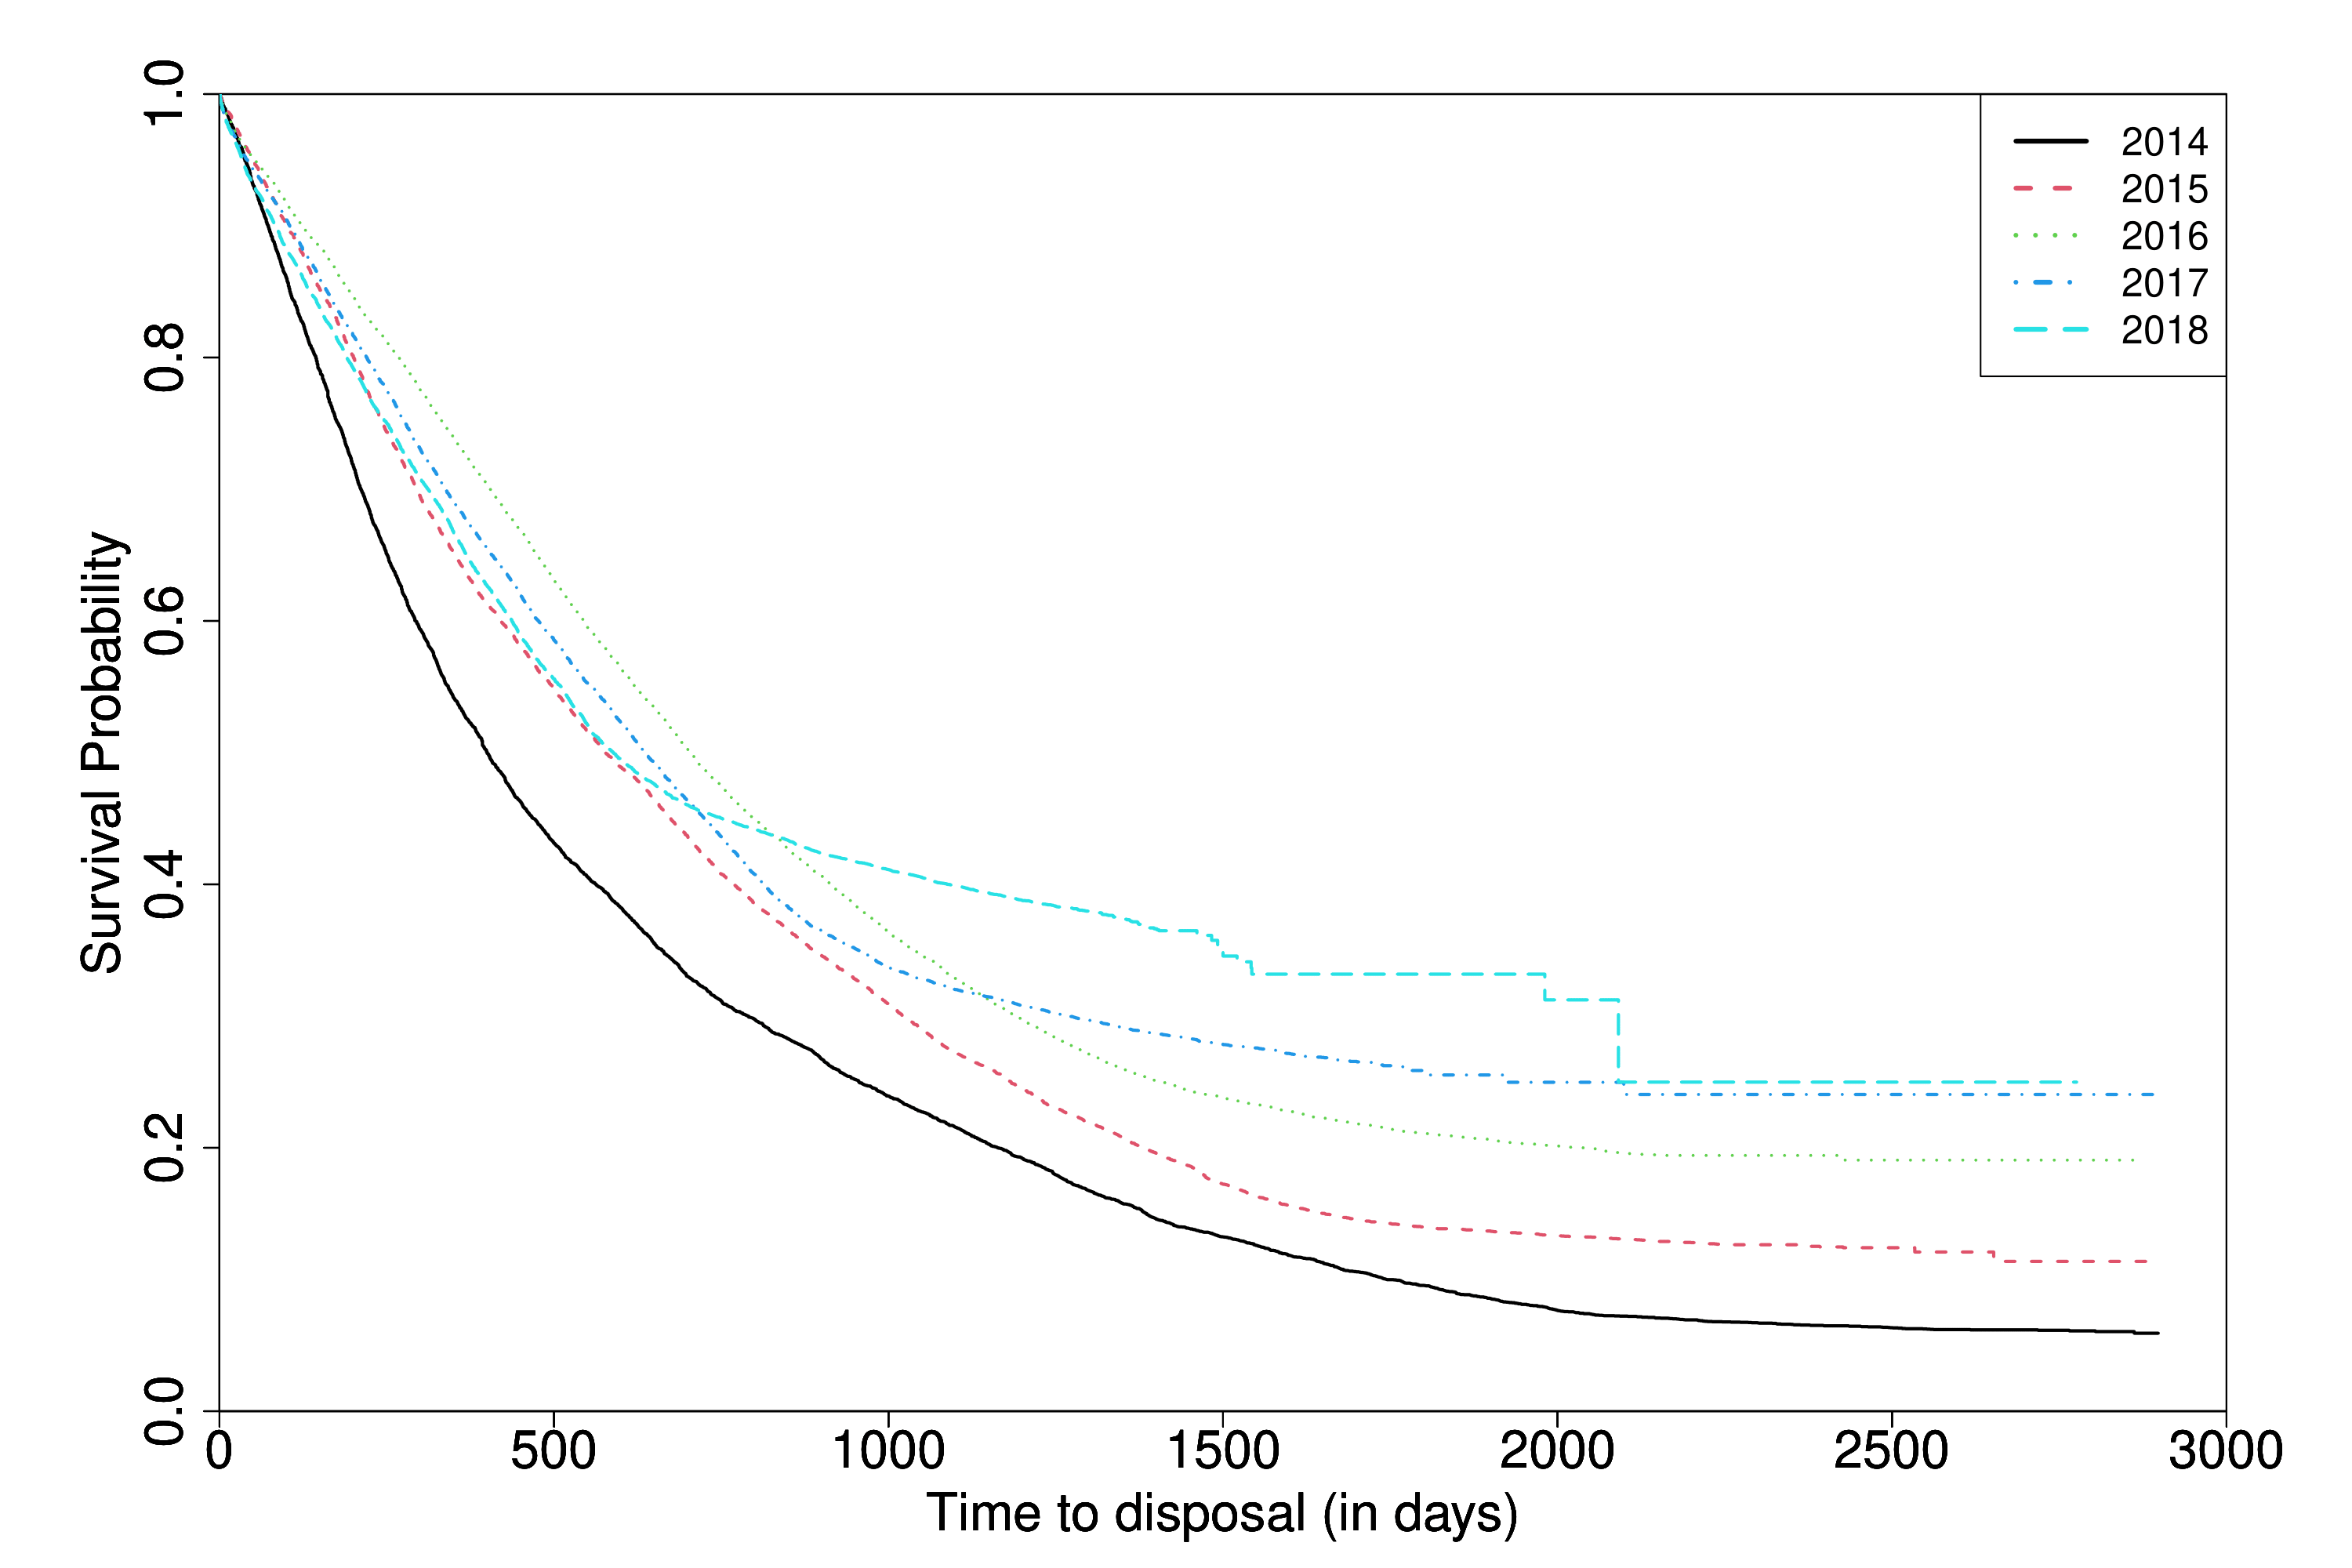
\includegraphics[width = 0.9\textwidth]{surv_years-1.png}
\end{figure}

{\footnotesize \begin{longtable}{lcc|ccc} 
 \caption{Disposal Days: Variation across years}\label{tab:yearFE}
 \\[-1.8ex]
 \hline \\[-1.8ex] 
 & \multicolumn{5}{c}{\textit{Dependent variable: Disposal days}} \\ 
 \cline{2-6} 
 \\[-1.8ex] & (2014) & (2015) & (2016) & (2017) & (2018)\\ 
 \hline \\[-1.8ex]
 
 D(non-Appearance) & 155.424$^{***}$ & 186.156$^{***}$ & 220.051$^{***}$ & 185.167$^{***}$ & 242.311$^{***}$ \\ 
 & (8.163) & (8.921) & (10.899) & (13.316) & (14.042) \\ 
 & & & & & \\ 
 D(Summons) & 35.087$^{***}$ & 29.933$^{***}$ & 118.444$^{***}$ & 182.578$^{***}$ & 220.014$^{***}$ \\ 
 & (8.335) & (8.710) & (11.340) & (14.351) & (17.025) \\ 
 & & & & & \\ 
 D(Mediation) & 61.687$^{***}$ & 37.802$^{***}$ & 76.600$^{***}$ & 156.578$^{***}$ & 255.746$^{***}$ \\ 
 & (7.862) & (8.316) & (10.465) & (13.797) & (17.196) \\ 
 & & & & & \\ 
 D(Jurisdiction) & 180.482$^{***}$ & 231.023$^{***}$ & 269.201$^{***}$ & 313.779$^{***}$ & 318.416$^{***}$ \\ 
 & (9.022) & (8.876) & (10.238) & (12.909) & (13.564) \\ 
 & & & & & \\ 
 D(Multiplicity) & 64.826$^{***}$ & 138.977$^{***}$ & 141.382$^{***}$ & 201.150$^{***}$ & 246.812$^{***}$ \\ 
 & (19.158) & (17.088) & (20.037) & (24.870) & (31.392) \\ 
 & & & & & \\ 
 D(Contested) & 5.510 & $-$12.717 & $-$59.490$^{***}$ & $-$75.624$^{***}$ & $-$71.797$^{***}$ \\ 
 & (10.927) & (10.419) & (11.695) & (12.818) & (13.581) \\

 \hline \\[-1.8ex]
 State FE & Y & Y & Y & Y & Y \\
 \hline \\[-1.8ex] 
 
 Observations & 6,760 & 8,458 & 8,165 & 6,117 & 5,927 \\ 
 R$^{2}$ & 0.189 & 0.202 & 0.228 & 0.232 & 0.269 \\ 
 Adjusted R$^{2}$ & 0.187 & 0.201 & 0.226 & 0.230 & 0.268 \\
 
 \hline \\[-1.8ex] 
 \multicolumn{6}{l}{\textit{Note:} $^{*}$p$<$0.1; $^{**}$p$<$0.05; $^{***}$p$<$0.01} \\
\end{longtable}
}



%%% Local Variables:
%%% mode: latex
%%% TeX-master: "paper_chequeDishonour"
%%% End:
